\section{Testing and development}

During the development of the type-level mathematical expression evaluator, several invaluable tools were discovered and utilised that significantly contributed to the implementation. This section is devoted to discussing these tools and their impact on the overall development process.

The core of the development experience is underpinned by TypeScript Standalone Server, also known as \code{tsserver}. \code{tsserver} encapsulates both the compiler and the accompanying language services for use in editors and \acrshort{ide}s, communicating via \acrshort{lsp} to add support for code completion, auto-importing, symbol renaming etc. \code{tsserver} also provides the ability to see the inferred types of any symbol by hovering on top the symbol, as seen in Figure \ref{fig:tsserver-hover}. This service is invaluable when developing a type-level library, as it allows the developer to break down complex types into smaller pieces, achieving better readability.

\begin{figure}[ht]
  \centering
  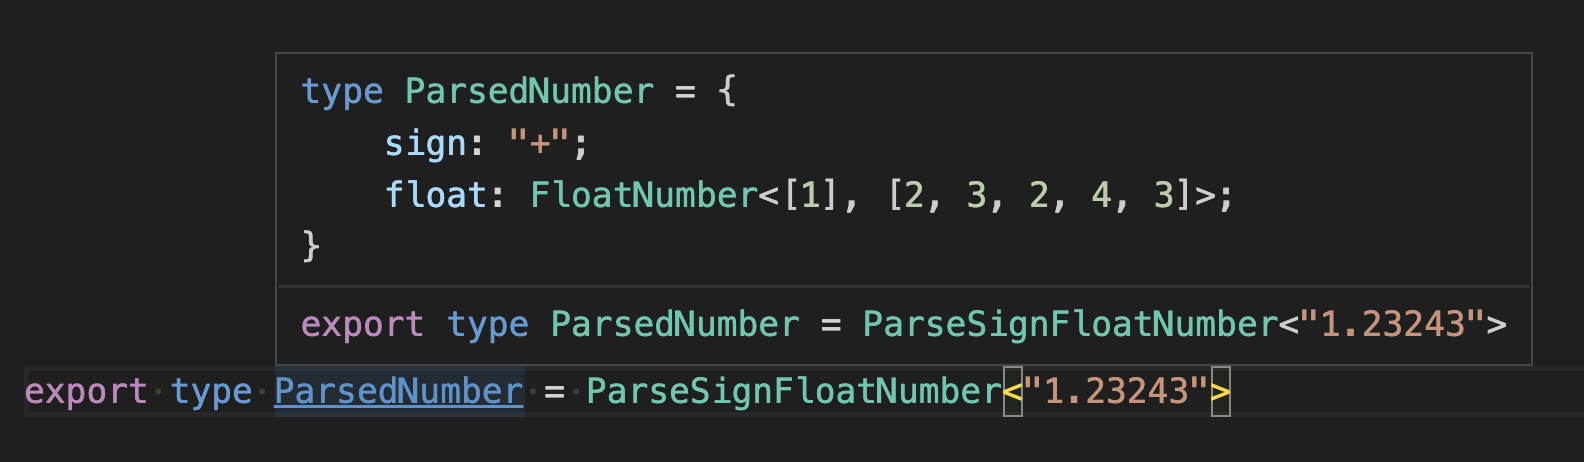
\includegraphics[width=\textwidth]{text/testing/tsserver-hover.png}
  \caption{Inferred type on hover in \acrshort{vscode}}
  \label{fig:tsserver-hover}
\end{figure}

Another critical tool used when developing the implementation is \code{vscode-twoslash-plugin} extension \cite{theroxVscodetwoslashqueries2023}. In order to avoid hovering the mouse over a symbol to see the inferred type, developers can write the \vcode{// ^?} comment, with the caret pointing to the targeted symbol. The plugin will then display an inlay hint with the inferred type of the selected symbol, as seen in Figure \ref{fig:twoslash-plugin}.

\begin{figure}[ht]
  \centering
  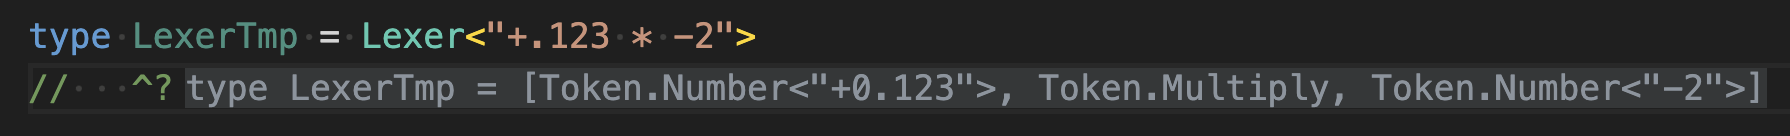
\includegraphics[width=\textwidth]{text/testing/vscode-twoslash-plugin.png}
  \caption{Twoslash syntax of \code{vscode-twoslash-plugin}}
  \label{fig:twoslash-plugin}
\end{figure}

Finally, Pretty TypeScript Errors \cite{balasianoPrettyTypeScriptErrors2023} attempts to parse and reformat the TypeScript error messages to be more human-readable in \acrshort{vscode}. This is especially helpful when dealing with complex object types, where the error messages can become unreadable since the error message and the serialised type is printed out on a single line, as seen in Figure \ref{fig:pretty-ts-errors}.


\begin{figure}[ht]
  \centering
  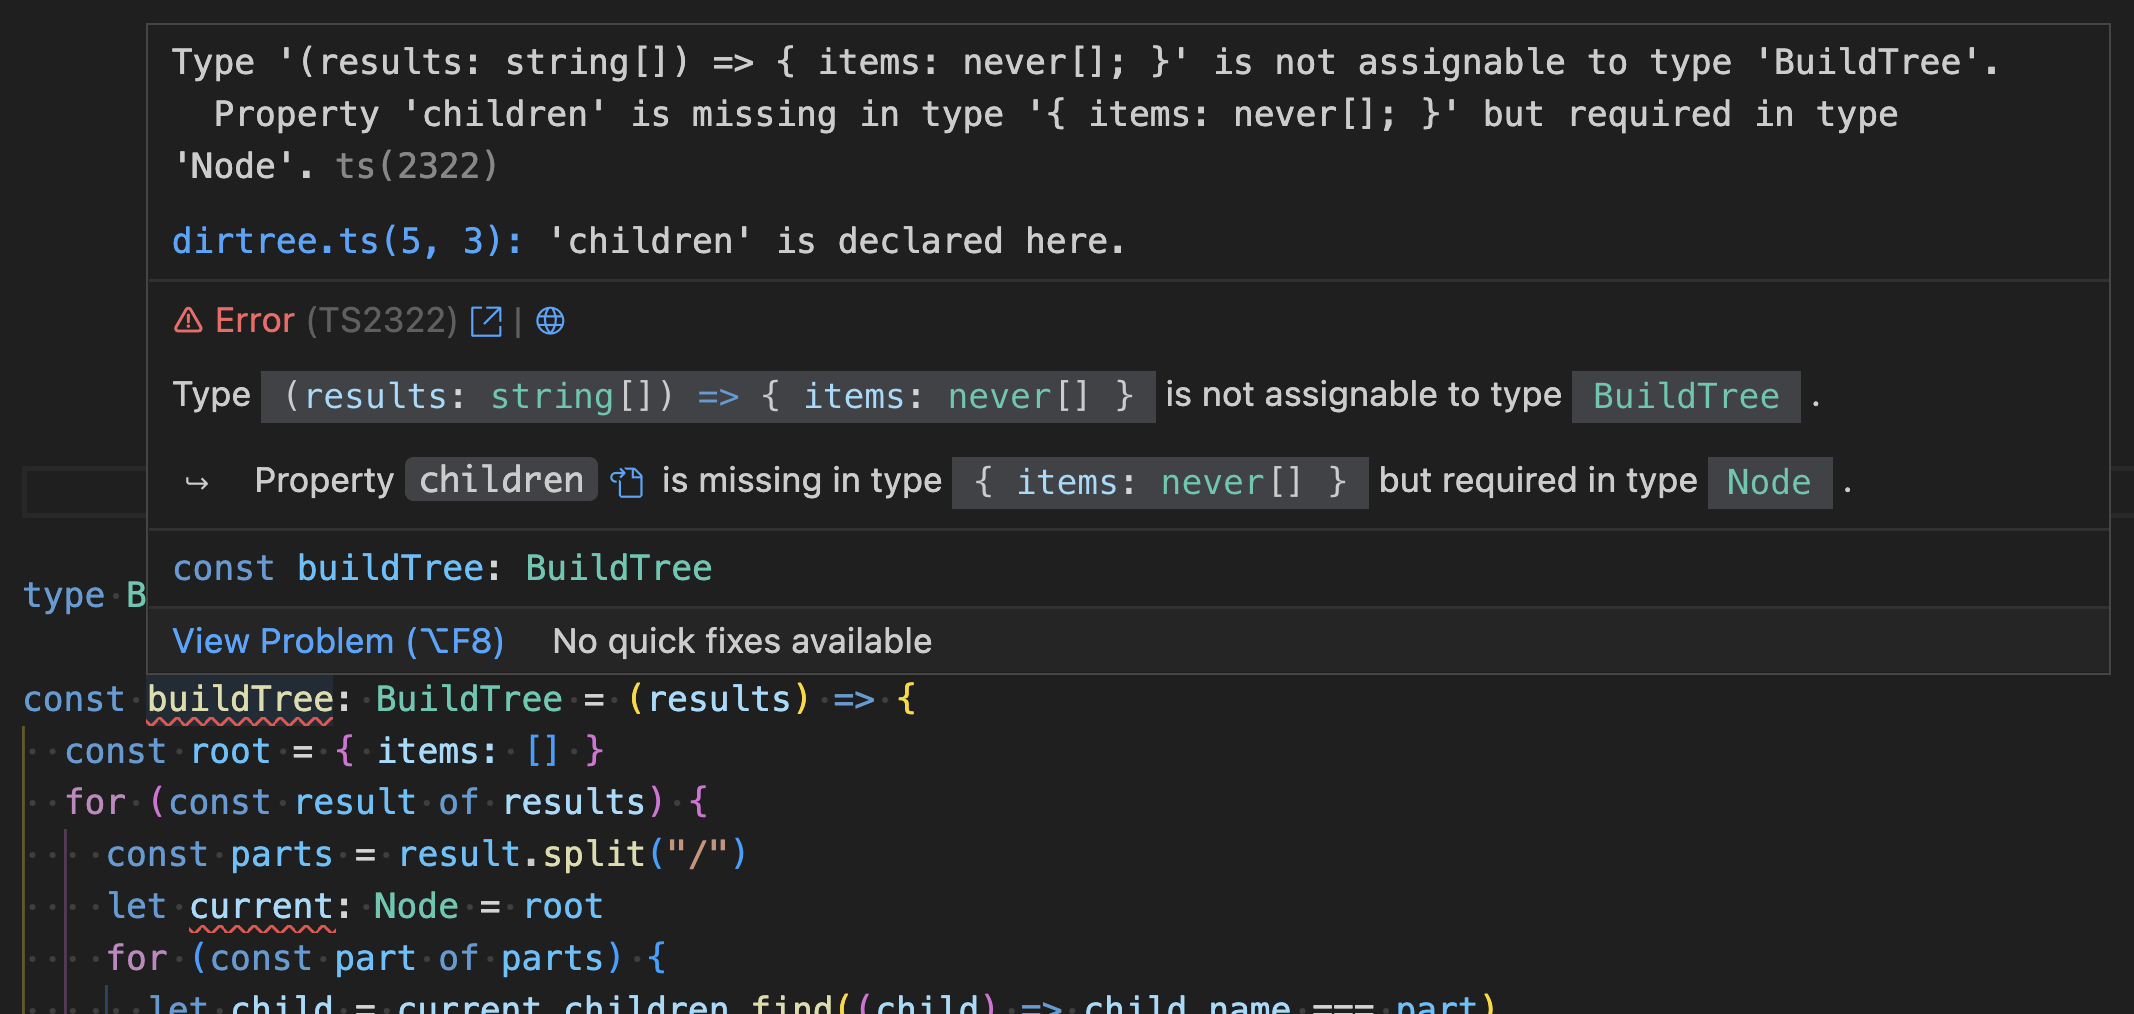
\includegraphics[width=\textwidth]{text/testing/pretty-ts-errors.png}
  \caption{Formatting errors with Pretty \acrshort{ts} Errors extension}
  \label{fig:pretty-ts-errors}
\end{figure}

Some generic types include an accompanying unit test to ensure correctness and prevent regression. Testing is backed with \code{eslint}\cite{ESLint2023}, a static code analyser for JavaScript and TypeScript. Configuration-wise, \code{@typescript-eslint/parser} has been set up as the parser used by ESLint for properly analysing TypeScript code, and \code{eslint-plugin-expect-type} has been added for writing type assertions as comments. \code{eslint-plugin-expect-type} enables writing \code{\$ExpectType}, \code{\$ExpectError} and twoslash type assertions (\vcode{// ^?}). An example test assertion can be seen in Listing \ref{lst:expect-type}.

\begin{listing}[ht]
  \caption{Type assertion with \code{\$ExpectType}}\label{lst:expect-type}
  \begin{minted}{TypeScript}
// $ExpectType "0.3619047620"
type EvaluateCase = Evaluate<
  RecursiveParser.Parse<Lexer<"3.1 + 2.5 * (1 - 5.6) / 4.2">>
>
\end{minted}
\end{listing}

Other testing frameworks, such as Jest or Vitest, have been considered for this thesis but ultimately rejected due to the lacklustre support for type-level assertions. These frameworks tend to output only the values mismatch errors without printing out the actual inferred type.

\todo{Validate this claim}